\section{Acquisto Hardware}
\labelsec{Hardware Procurement}

Sfortunatamente il primo problema incontrato in un progetto come il seguente e' stata la necessit\'a di acquistare la parte hardware del sistema che si andr\' a costruire. Di consequenza si e' messo in atto un processo di ricerca dei sensori, cavi e quant'altro per riuscire a soddisfare i requisiti

\subsection{Dispositivi di Computazione}

Prima di tutto necessitiamo di un dispositivo in grado di computare i dati emessi dai vari sensori e che sia interamente programmabile. Nel corso abbiamo visto due possibilita' che hanno avuto molto successo recentemente:

\begin{itemize}
  \item Arduino
  \item Raspberry Pi
\end{itemize}

Abbiamo scelto la seconda opzione data la maggior familiarita' con il dispositivo e dal momento in cui risulta piu' facile il riutilizzo dello stesso una volta terminato questo progetto.

\begin{figure}
\centering
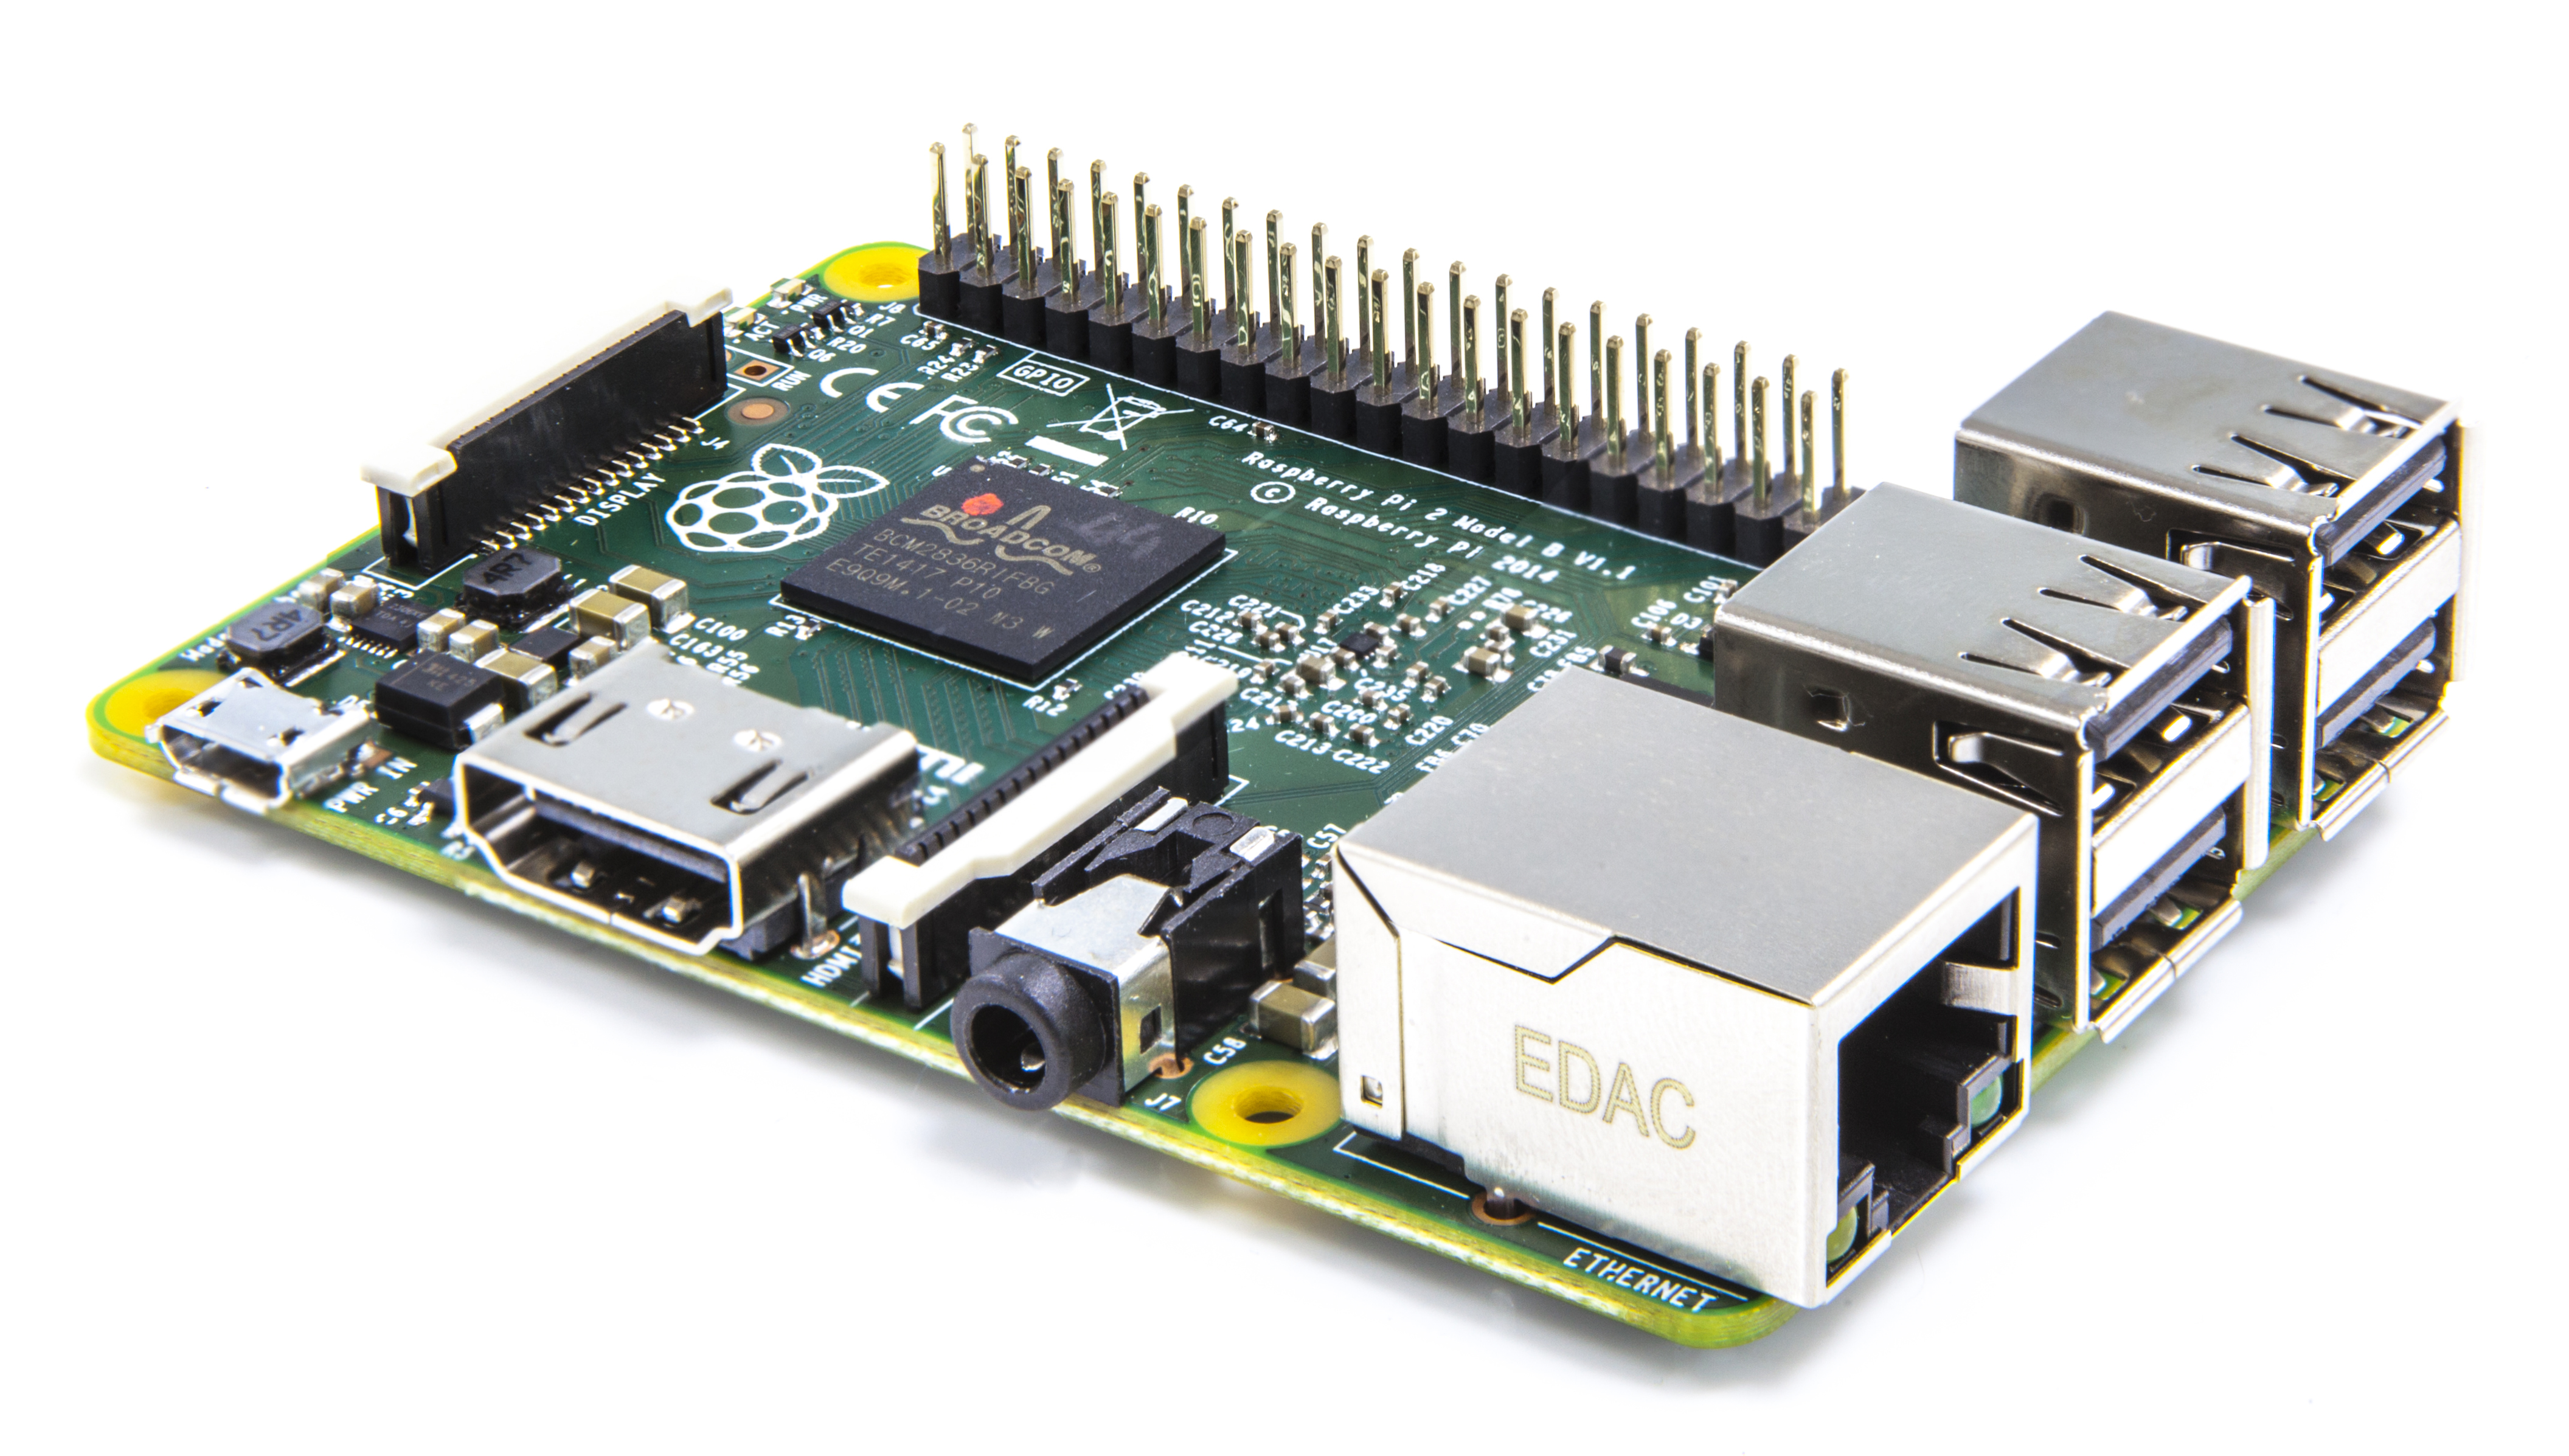
\includegraphics[width=0.7\linewidth]{Figures/Sensors&Rasp/Pi2}
\caption[raspberry]{Scheda del Raspberry 2}
\label{fig:Pi2}
\end{figure}



Il Rasberry Pi 2 (rappresentato nell'immagine~\ref{fig:Pi2}) è un SoC (sistema integrato) cio\'e possiede un chip che integra al suo interno processore, chipset, RAM ed eventuale circuteria input/output. \'E dotato delle seguenti uscite:
\begin{itemize}
\item USB 2.0 (4)
\item Ethernet
\item HDMI
\item Aux
\item DC (Alimentazione)
\item Slot MicroSD
\end{itemize}
Infine dispone di un GPIO (General Purpose Input/Output) interfaccia attraverso la quale è possibile comunicare con sensori esterni per mezzo di segnali digitali ed interagire con l'ambiente esterno.

Costo del dispositivo: 44,50 \euro

\subsection{Sensori}

Un'altra cosa fondamentale riguarda i sensori necessari per catturare i parametri richiesti.
Tutti i sensori per standard possono lavorare con una tensione di 5v.
Ogni sensore possiede 3 o 4 pin:

\begin{itemize}
	\item Vcc: Pin di alimentazione
	\item GND: Pin della massa
	\item Dout: Porta input/output digitale
	\item Aout: Porta input/output analogica (opzionale)
\end{itemize}

 Abbiamo Quindi scelto i sequenti sensori:

\begin{table}[]
	
	\begin{tabular}{lllll}
		\cline{1-3}
		\multicolumn{1}{|l|}{Parametri Ambientali} & \multicolumn{1}{l|}{Sensori} & \multicolumn{1}{l|}{Costo} &  &  \\ \cline{1-3}
		Temperatura \& Umidità                     & DHT11                        & 6\euro                          &  &  \\
		Luminosità                                 & Light                        & 5\euro                          &  &  \\
		Movimento                                  & HC-SR501                     & 6\euro                          &  &  \\
		Gas                                  & MQ-2                   & 7\euro                         &  &
	\end{tabular}
	\centering
	\caption{Sensor table}
	\label{my-label}
	
\end{table}

\begin{figure}
\centering
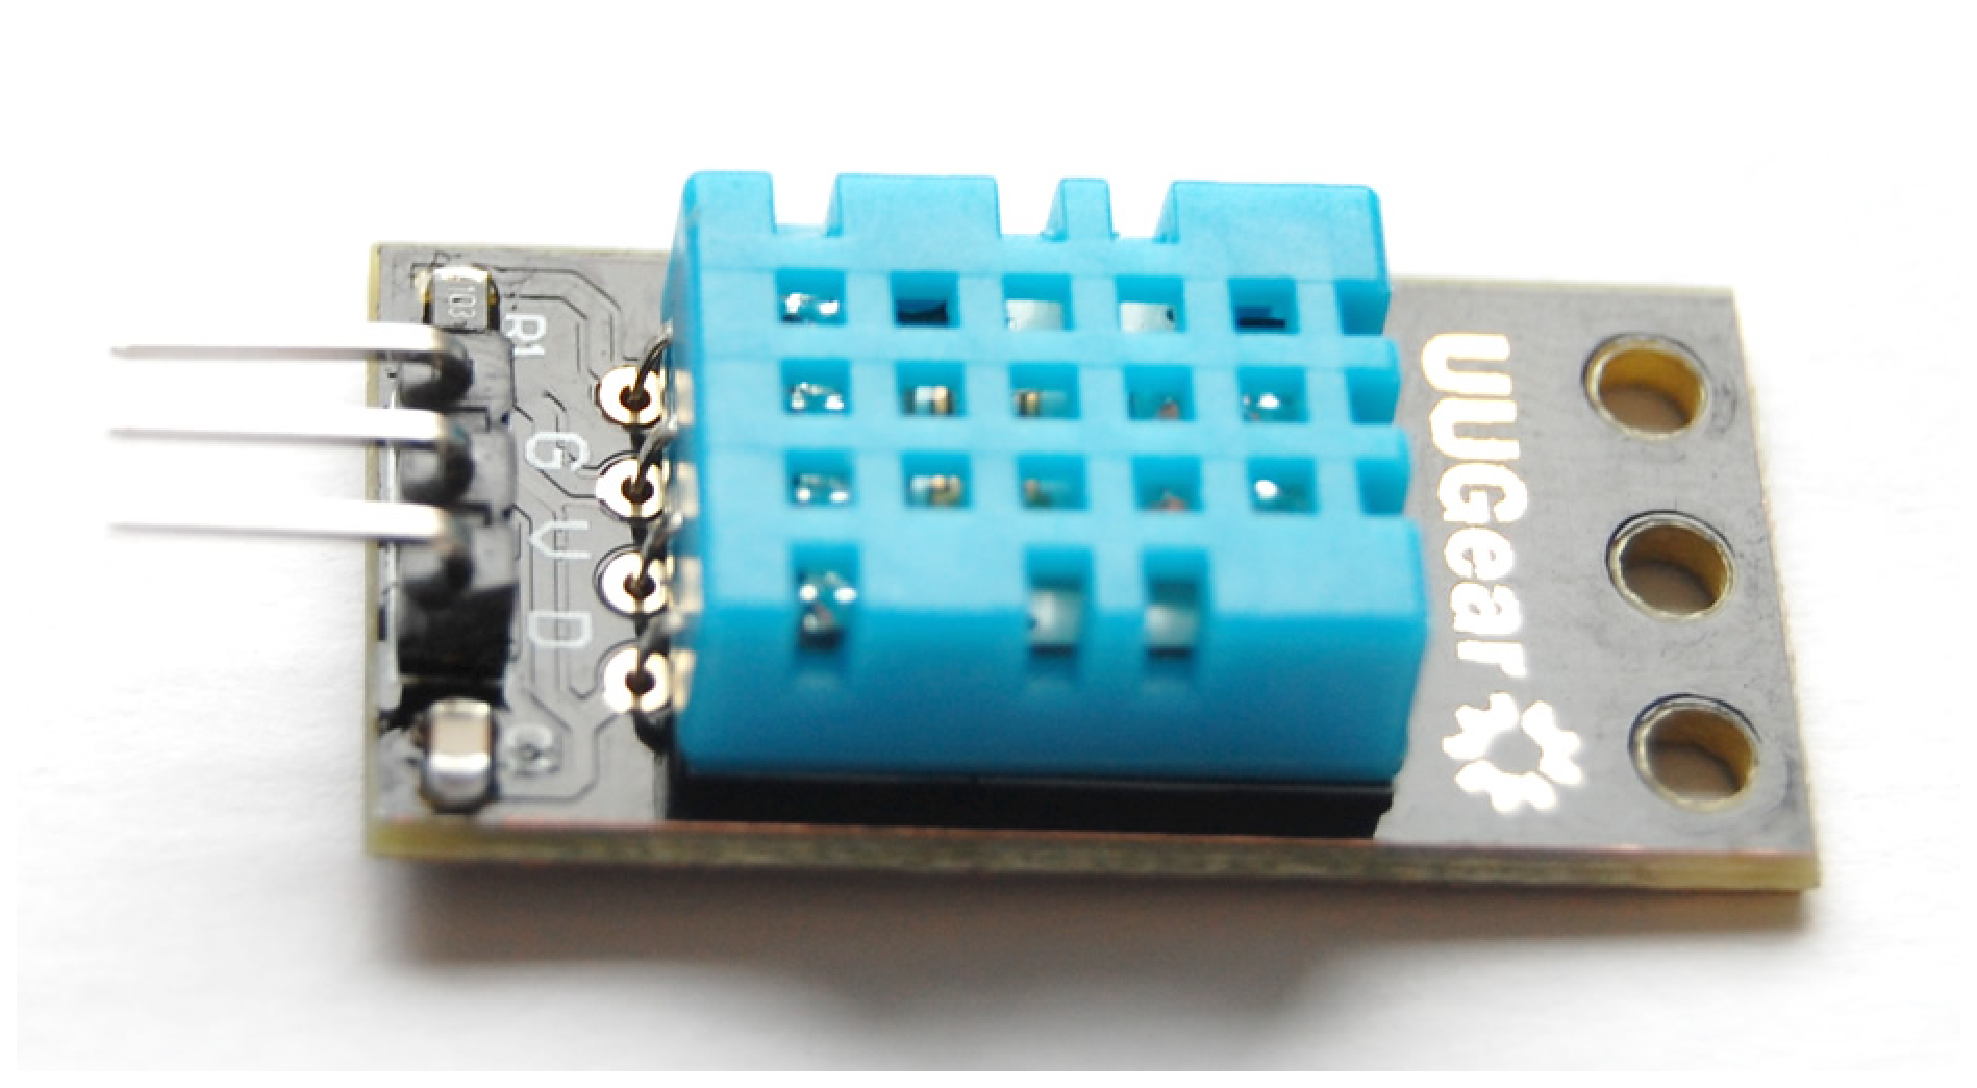
\includegraphics[width=0.7\linewidth]{Figures/Sensors&Rasp/dht11}
\caption[dht11]{DHT11 Sensor}
\label{fig:dht11}
\end{figure}

 Il sensore DHT11 è in grado rilevare la temperatura e l'umidità dell'ambiente circostante. Possiede 3 Pin per interfacciarsi.
 Le sue caratteristiche tecniche sono:
 
 \begin{itemize}
 	\item Vcc: 3.3~5.5V
 	\item Range: Temperatura 0 \textasciitilde 50℃, Umidità:  20-90%RH
 	\item Accuratezza: Temperatura +-2℃, Umidit\'a +-5%RH
 	\item Risoluzione: Temperatura  1℃, Umidit\'a  1%RH
 \end{itemize}
 


\begin{figure}
	\centering
	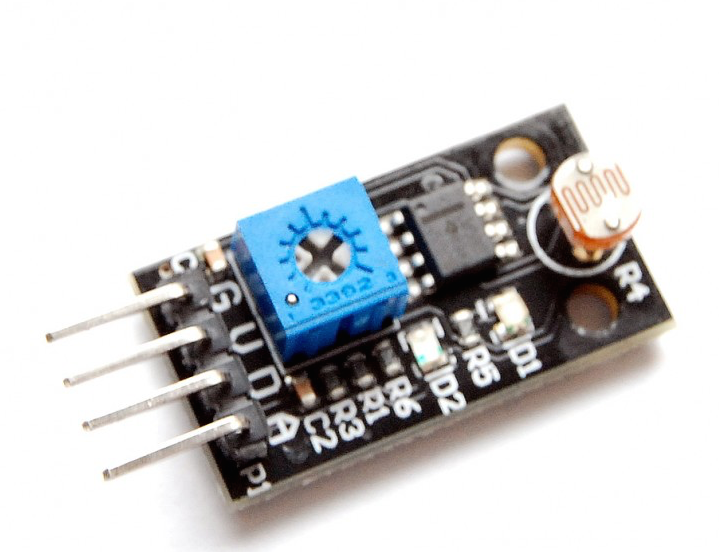
\includegraphics[width=0.7\linewidth]{Figures/Sensors&Rasp/light}
	\caption[light]{Light Sensor}
	\label{fig:dht11}
\end{figure}
\begin{figure}
	\centering
	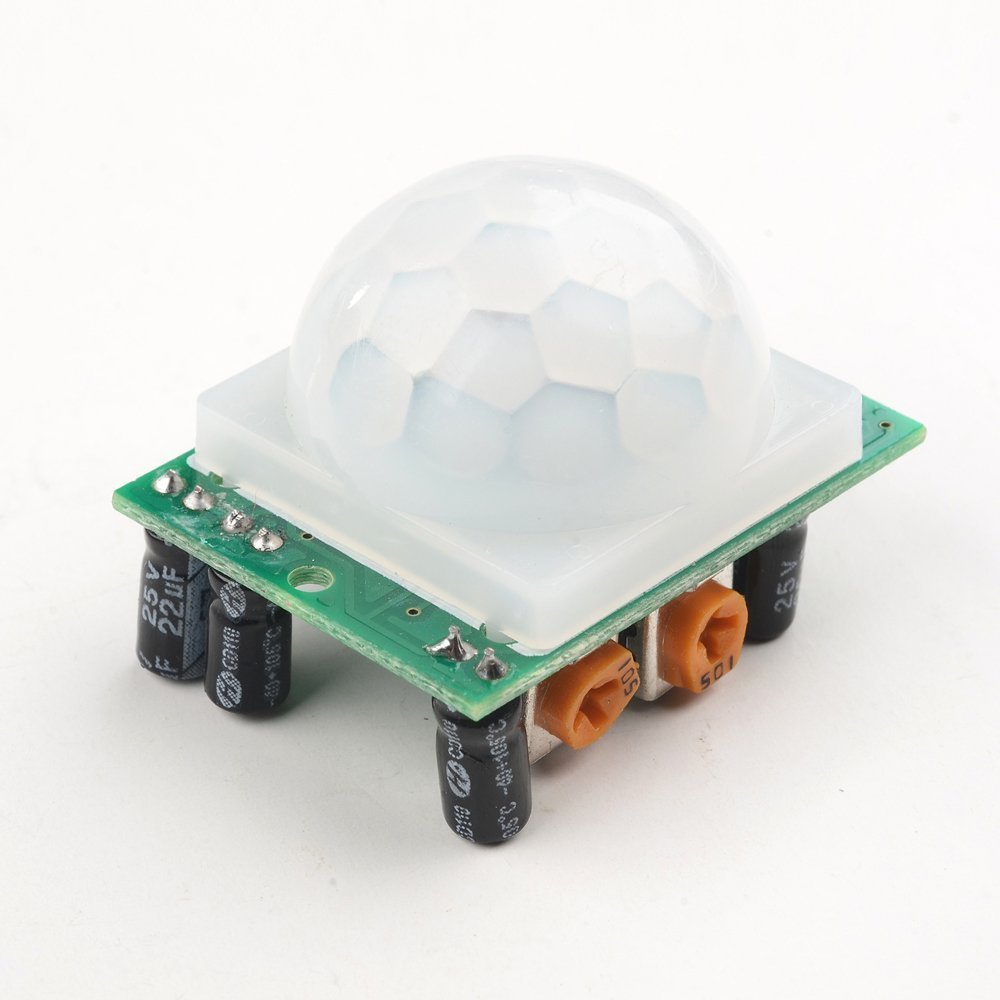
\includegraphics[width=0.7\linewidth]{Figures/Sensors&Rasp/pir}
	\caption[pir]{PIR (HC-SR501) Sensor}
	\label{fig:dht11}
\end{figure}
\begin{figure}
	\centering
	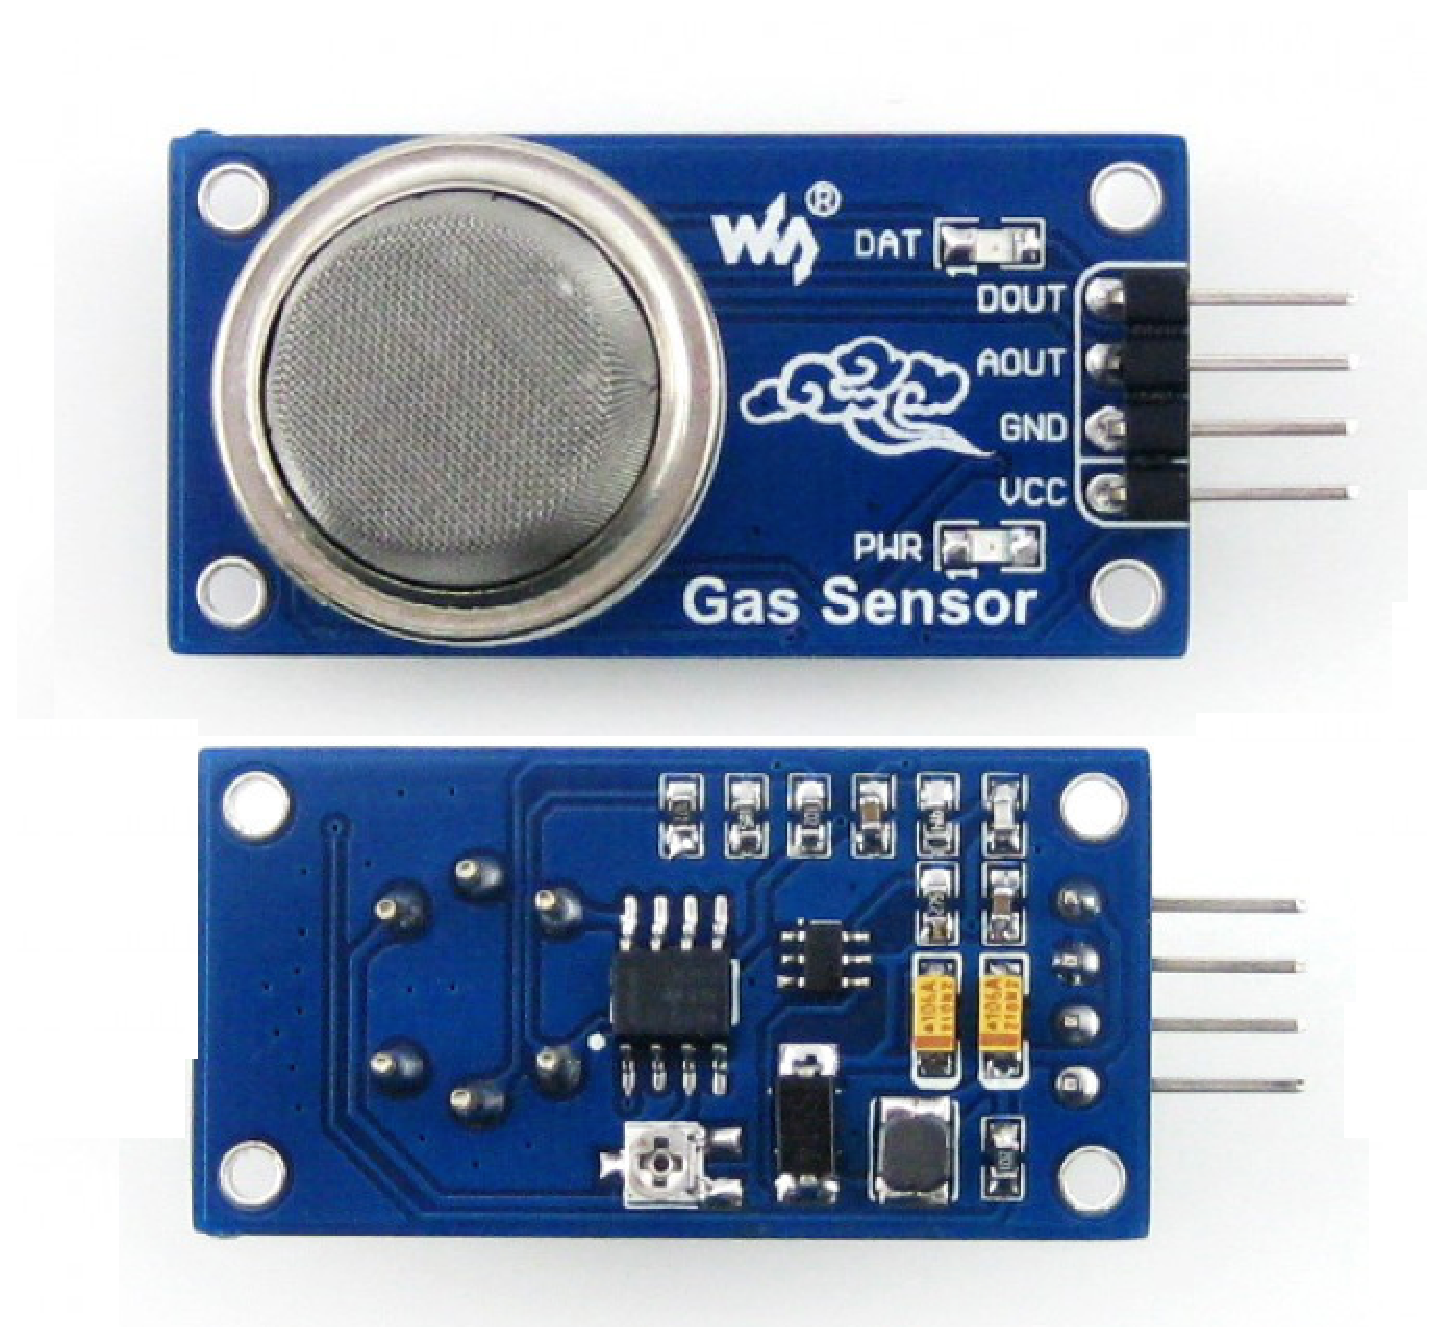
\includegraphics[width=0.7\linewidth]{Figures/Sensors&Rasp/mq-2}
	\caption[gas]{Gas sensor (MQ-2)}
	\label{fig:dht11}
\end{figure}




\subsection{Hardware Aggiuntivo}

\begin{table}[]
\centering
\begin{tabular}{lll}
\multicolumn{1}{c}{\textbf{Hardware}} &  & \multicolumn{1}{c}{\textbf{Costo}} \\
Wires                                 &  &                   8\euro                \\

\end{tabular}
\caption{Addictional Hardware}


\label{Addictional Hardware}
\end{table}

\newpage
